\chapter{基于集中平台的iBGP系统结构}
\label{cha:architecture}


\section{本章引言}
可扩展问题是互联网iBGP协议的重要问题,随着网络规模和需求的不断增加,大多数自治系统已经不采用传统的Full-Mesh的iBGP连接结构,而是使用配置比较方便、技术比较成熟的路由反射。现有的解决iBGP可扩展问题的思路可分为两种:分布式路由体系结构、集中式路由体系结构。分布式路由体系结构下的相关研究主要有路由反射和AS联邦,其解决了iBGP的可扩展问题,但是带来了新的问题,比如:非最优出口、转发环路、路由震荡。而集中式路由体系结构的相关研究主要有SoftRouter、RCP、RFCP三种代表性方案,这三种方案解决了iBGP的可扩展问题,但也分别存在集中平台本身的可扩展性差、路由存储冗余重复、未优化的传统路由计算方式等问题。

本文基于路由决策、存储集中化的思路,提出了基于集中平台的iBGP系统结构,将自治系统内部的路由存储、策略管理、路由计算以及路由转发交换功能合理划分到集中平台上运行的路由器和自治系统内边界路由器上分别执行。该基于集中平台的新型iBGP系统RSCP-iBGP系统,处理路由信息的基本流程如图\ref{fig:rscp-ibgp1},主要环节如下:
\begin{itemize}
  \item 自治系统内的边界路由器从某eBGP邻居收到路由信息,如果本地路由器配置了需要保存从该邻居过来的路由信息,则保存该路由信息到Adj-RIB-In。经过入站策略后,将过滤更新的路由通过扩展的iBGP协议发送到集中平台;
  \item 集中平台将收到的路由信息存入Loc-RIB、为每台自治系统内的边界路由器计算出最优路由,将最优路由通过iBGP协议发送给边界路由器;
  \item 每台边界路由器收到集中平台的最优路由,进行出站过滤,边界路由器将收到的路由信息通过eBGP连接宣告给所有的eBGP邻居。如果本地路由器配置了需要保存向某邻居宣告的路由信息,则将向外宣告的路由存入邻居对应的Adj-RIB-Out。
\end{itemize}

\begin{figure}
  \centering
  % Requires \usepackage{graphicx}
  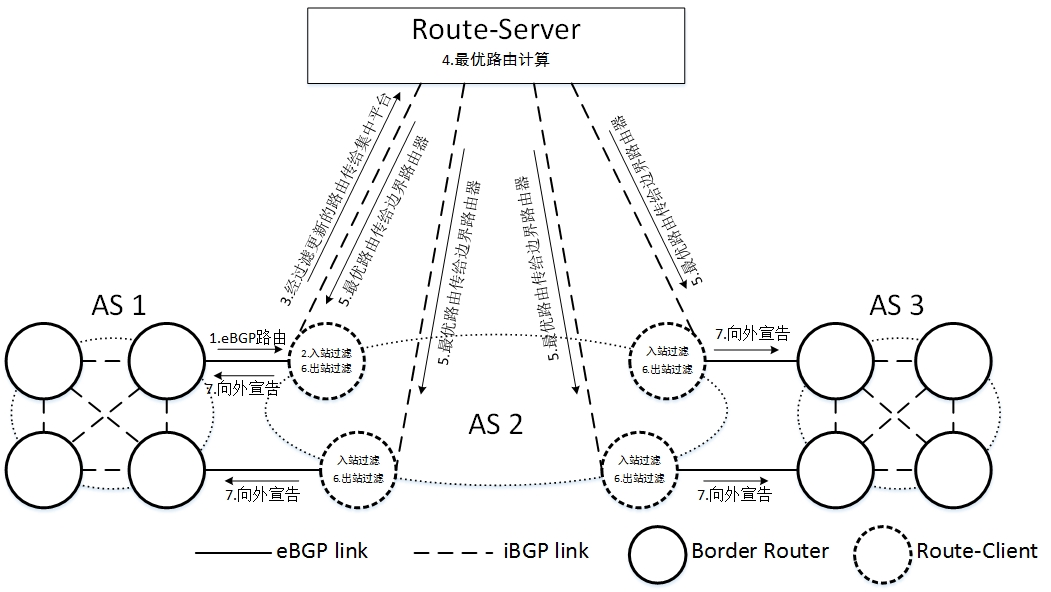
\includegraphics[width=\textwidth]{rscp-ibgp1}
  \caption{RSCP-iBGP系统逻辑流程图}
  \label{fig:rscp-ibgp1}
\end{figure}

集中式路由体系结构下,路由存储、策略管理、路由计算等存在很多优化空间。本文提出的基于集中平台的新型iBGP系统RSCP-iBGP,不仅解决了iBGP存在的可扩展问题,而且对自治系统内iBGP的路由存储和路由计算进行了优化。

本章首先提出基于集中平台的新型iBGP系统RSCP-iBGP的系统架构图,之后对系统中的三个主要组成部分(边界路由器、集中平台、边界路由器与集中平台的通信协议)进行了详细的介绍,最后从解决iBGP可扩展问题、与分布式路由体系结构方案的对比、与集中式路由体系结构方案的对比等方面对基于集中平台的RSCP-iBGP系统进行了定性的分析。

\section{新型iBGP路由系统}
本文提出的自治系统内部的基于集中平台的iBGP新架构命名为RSCP-iBGP(Route Server Control Platform iBGP)。RSCP-iBGP的基本思想是将自治系统内边界路由器的控制平面和数据平面进行部分分离,将边界网关协议BGP中的路由计算、Loc-RIB路由存储从边界路由器中剥离出来,交由独立的、且逻辑比较集中的运行在集中平台的Route-Server执行或存储,而自治系统内部的普通边界路由器作为Route-Client对路由信息进行接收转发、入站出站过滤更新、Adj-RIBs-In和Adj-RIBs-Out存储等操作。

RSCP-iBGP系统架构如图\ref{fig:rscp-ibgpnew},这个系统运行在自治系统内部,主要包含三部分:自治系统内部的集中平台(Route-Server),自治系统内部的多台边界路由器(Route-Client),以及自治系统内部边界路由器与集中平台的通信协议(扩展的iBGP协议)。

\paragraph{RSCP-iBGP系统中的集中平台} 集中平台上运行1台Route-Server进行集中式的路由存储、路由计算。当Route-Server上的接收iBGP路由模块,收集到自治系统内部边界路由器Route-Client-Ri发来的更新路由消息,Route-Server先将该路由输入Loc-RIB增量存储模块,存储经过入站策略的路由信息,将Loc-RIB表等相关信息输入到路由复式计算模块,得到自治系统每台边界路由的针对该前缀的最优路由,将其结果输入到宣告iBGP路由模块,分别将未经出站过滤策略的该前缀的最优路由传输给自治系统内的每台边界路由器。

\paragraph{RSCP-iBGP系统中的边界路由器} 该新型iBGP系统中的边界路由器收到不同的路由信息,进行不同的处理流程:

\begin{itemize}
    \item 当收到其他自治系统发来的eBGP路由时,根据收到路由eBGP邻居的配置,决定是否将其存储到对应eBGP邻居的Adj-RIB-In。边界路由器Route-Client将收到的路由信息进行入站策略的过滤更新,将得到的路由通过扩展的iBGP协议(携带Weight属性)发送给集中平台上的Route-Server;
    \item 当收到集中平台上的Route-Server发来的iBGP路由时,边界路由器Route-Client将收到的路由信息进行出站策略的过滤更新,将经过出战策略的路由其宣告给自己的所有eBGP邻居,同时根据对应的eBGP邻居的配置,决定是否将其存储到对应eBGP邻居的Adj-RIB-Out。
\end{itemize}

\paragraph{RSCP-iBGP系统中的通信协议} 通信协议使用扩展的iBGP协议,来传输BGP路由信息。在扩展的iBGP协议中,边界路由协议需要将携带Weight属性值的路由更新报文传输到集中平台上的Route-Server路由器,集中平台收到之后需要对该报文的路由信息(包括新添加的路径属性Weight的相关信息)进行正确的解析。

\begin{figure}
  \centering
  % Requires \usepackage{graphicx}
  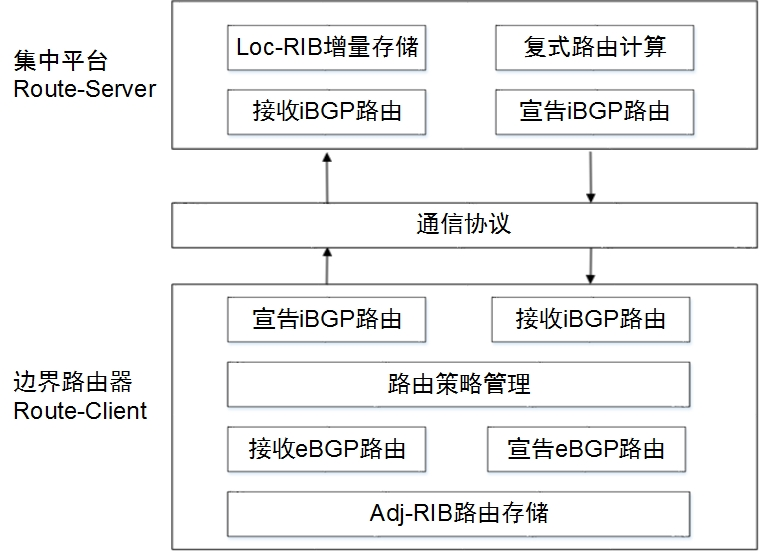
\includegraphics[width=0.8\textwidth]{rscp-ibgpnew}
  \caption{RSCP-iBGP系统架构图}
  \label{fig:rscp-ibgpnew}
\end{figure}

\section{系统详细介绍}
本文提出的新型RSCP-iBGP系统,主要包含三大部分:集中平台、边界路由器、通信协议,本小节将对这三个部分进行详细介绍。
\subsection{集中平台}
\subsubsection{Loc-RIB增量存储模块}

\begin{figure}
  \centering
  % Requires \usepackage{graphicx}
  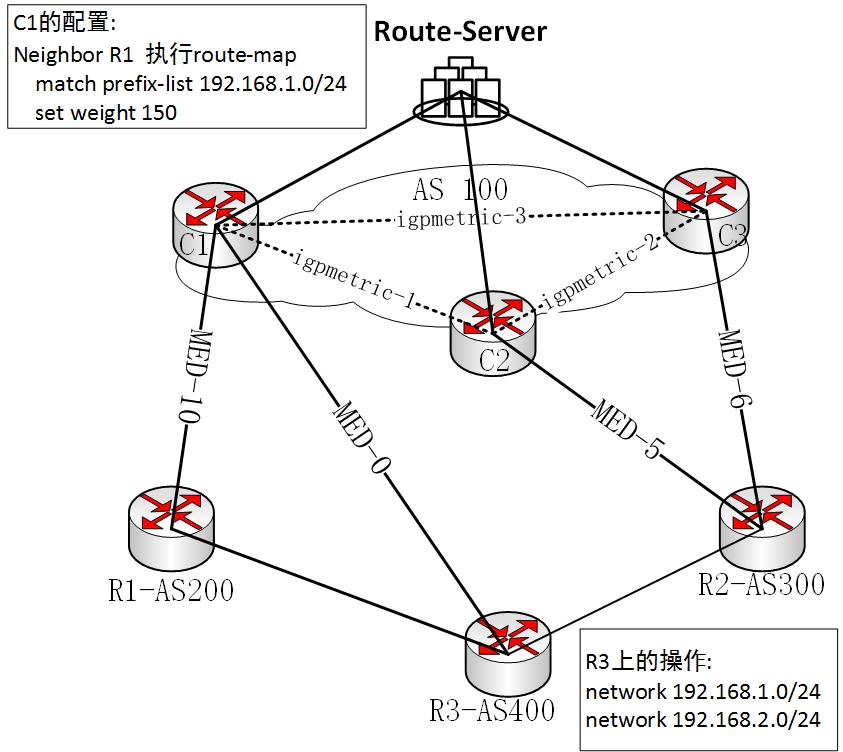
\includegraphics[width=0.7\textwidth]{rscp-example1}
  \caption{Loc-RIB增量存储案例使用的网络拓扑图}
  \label{fig:rscp-example1}
\end{figure}

传统网络中,自治系统的边界路由器收到从eBGP邻居传来的更新路由信息,该边界路由器会将该路由信息经过入站策略后更新到Loc-RIB表,选择最优路由宣告给其iBGP邻居。早期自治系统内的边界路由器建立Full-Mesh的iBGP连接,以此来使得外界的路由信息传输到自治系统内部的每台边界路由器。路由经过入站策略后,可能传输到每台边界路由器会有所差异,但大部分前缀在大部分边界路由器上的Loc-RIB表的路由信息都基本相同。入站策略和出站策略主要用于eBGP路由的过滤更新,传统的iBGP策略大多仅配置next-hop-self(通过设置next-hop-self将iBGP协议UPDATE报文中传输的next-hop值修改为iBGP邻居的IP地址,从而保证路由的可达性)。根据BGP协议的特性以及网络中路由表的存储实现,本文提出了Loc-RIB增量存储的概念。

综合本文第二章对BGP的路由策略、路由计算的综述,可以发现在自治系统内,对于特定的前缀,Weight和IGPcost两个路径属性是影响每台边界路由器与其他边界路由器最优路由不同的关键因素。Weight路由属性仅本地路由器有效,不传输给其他的边界路由器。不同边界路由器到其他边界路由器的IGPcost并不相同。仅从路由存储的角度考虑,可以在集中平台上的Route-Server中存储一份Public-Loc-RIB。此外,针对每个iBGP的对等体,Route-Server路由器存储曾配置过Weight值的Prefix的所有路由表项(因为Weight仅在本地路由器有效,并不会影响其他边界路由器的选路,属于边界路由器特有的路由信息,需要单独存储)。Loc-RIB增量存储中增量的含义为,将每台边界路由器特有的路由信息增量存储。为了便于该边界路由器前缀最优路由的计算,将该边界路由器可能受到Weight值影响的前缀的所有路由增量存储。



%\begin{table}[h]
%	\centering
%	\caption{Route-Server上存储的Public-Loc-RIB路由信息}
%    \label{tab:weight-example}
%	\begin{tabular}{|c|c|c|c|c|c|c|}
%		\hline
%		network & received-peer & metric & LocPrf & Weight & Path & ebgp-next-hop \\ \hline
%		192.168.1.0 & C1 & 0 & & / &400,i & R3 \\ \hline
%        192.168.1.0 & C1 & 10 & & / &200,400,i & R1 \\ \hline
%        192.168.1.0 & C2 & 5 & & / &300,400,i & R2 \\ \hline
%        192.168.1.0 & C3 & 6 & & / &300,400,i & R2 \\ \hline
%        192.168.2.0 & C1 & 0 & & / &400,i & R3 \\ \hline
%        192.168.2.0 & C1 & 10 & & / &200,400,i & R1 \\ \hline
%        192.168.2.0 & C2 & 5 & &  /&300,400,i & R2 \\ \hline
%        192.168.2.0 & C3 & 6 & & / &300,400,i & R2 \\ \hline
%	\end{tabular}
%\end{table}

\begin{table}[h]
	\centering
	\caption{Route-Server上存储的Public-Loc-RIB路由信息}
    \label{tab:weight-example}
    \begin{tabular}{@{}ccccccc@{}}
    \toprule
    Network     & Received-peer & Metric & LocPrf & Weight & Path      & Ebgp-next-hop \\ \midrule
    192.168.1.0 & C1            & 0      &        & /      & 400,i     & R3            \\
    192.168.1.0 & C1            & 10     &        & /      & 200,400,i & R1            \\
    192.168.1.0 & C2            & 5      &        & /      & 300,400,i & R2            \\
    192.168.1.0 & C3            & 6      &        & /      & 300,400,i & R2            \\
    192.168.2.0 & C1            & 0      &        & /      & 400,i     & R3            \\
    192.168.2.0 & C1            & 10     &        & /      & 200,400,i & R1            \\
    192.168.2.0 & C2            & 5      &        & /      & 300,400,i & R2            \\
    192.168.2.0 & C3            & 6      &        & /      & 300,400,i & R2            \\ \bottomrule
    \end{tabular}
\end{table}

在图\ref{fig:rscp-example1}的拓扑中,ASN(Autonomous System Number,自治系统号)为100的自治系统在部署RSCP-iBGP系统的条件下,在Route-Server中Loc-RIB采用增量存储的方案。AS100中有3台Route-Client作为边界路由器,分别命名为C1、C2、C3。在C1上配置入站策略(C1从R1收到的前缀为192.168.1.0/24的路由将其Weight设置为150)。



%\begin{table}[h]
%	\centering
%	\caption{Route-Server上存储的针对C1的Pravite-Loc-RIB路由信息}
%    \label{tab:c1-loc-rib}
%	\begin{tabular}{|c|c|c|c|c|c|c|}
%		\hline
%		network & received-peer & metric & LocPrf & Weight & Path & ebgp-next-hop \\ \hline
%		192.168.1.0 & C1 & 0 & &  &400,i & R3 \\ \hline
%        192.168.1.0 & C1 & 10 & & 150 &200,400,i & R1 \\ \hline
%        192.168.1.0 & C2 & 5 & &  &300,400,i & R2 \\ \hline
%        192.168.1.0 & C3 & 6 & &  &300,400,i & R2 \\ \hline
%	\end{tabular}
%\end{table}


\begin{table}[h]
	\centering
	\caption{Route-Server上存储的针对C1的Pravite-Loc-RIB路由信息}
    \label{tab:c1-loc-rib}
	\begin{tabular}{@{}ccccccc@{}}
    \toprule
    Network     & Received-peer & Metric & LocPrf & Weight & Path      & Ebgp-next-hop \\ \midrule
    192.168.1.0 & C1            & 0      &        &        & 400,i     & R3            \\
    192.168.1.0 & C1            & 10     &        & 150    & 200,400,i & R1            \\
    192.168.1.0 & C2            & 5      &        &        & 300,400,i & R2            \\
    192.168.1.0 & C3            & 6      &        &        & 300,400,i & R2            \\ \bottomrule
   \end{tabular}
\end{table}

当R3向外宣告两条路由192.16.1.0/24和192.168.2.0/24,Route-Server收到了C1、C2、C3转发过来的路由信息,其存储的Public-Loc-RIB如表\ref{tab:weight-example}。因为集中平台上有自治系统内边界路由器与其他自治系统连接的网络拓扑,则 received-peer通过ebgp-next-hop的IP地址判断。因为前缀为192.168.1.0/24的通过C1传输到集中平台的两条路由,均需经过C1的入站策略,C1传输过来的ebgp-next-hop为R1且Weight值为150的路由信息,可能影响之后的路由决策,则需要单独存储从C1转发过来的192.168.1.0/24的所有路由,其存储的Private-Loc-RIB如表\ref{tab:c1-loc-rib}。


从表\ref{tab:weight-example}、表\ref{tab:c1-loc-rib}可以看出,Loc-RIB的增量更新方案对于减少Loc-RIB表的存储非常有效。如果自治系统内有N台边界路由器,传统的分布式路由体系结构下需要存储N张Loc-RIB表,而RSCP-iBGP系统中仅需存储1张Loc-RIB表,加m条单独的路由。RSCP-iBGP系统下自治系统内的Loc-RIB表占用存储空间的大小下降了一个数量级。


\subsubsection{复式路由计算}

传统的路由计算是分布式的路由计算,在每台边界路由器上输入一张Loc-RIB表,通过将更新前缀的全部路由根据更新时间由近到远两两比较,得到最优路由,属于单输入单输出的传统路由计算方法。而复式路由计算方法中,将所有路由器收到的路由信息Public-Loc-RIB以及多个存储部分前缀的Private-Loc-RIB作为复式计算的输入,得到针对特定前缀的自治系统内所有边界路由器的最优路由,属于多输入多输出的路由计算。

复式路由计算方法的基本思想是将前缀对应边界路由器的最优路由可能收到Weight值影响的,单独计算最优路由。遍历所有边界路由器的Private-Loc-RIB,如果存在该Prefix,则单独计算该边界路由器的针对该Prefix的最优路由,并以此结果为准。没有单独存储该Prefix路由的其他边界路由器,针对特定前缀Prefix,利用集中平台上的Public-Loc-RIB和IGPcosts, 计算出最优路由。

我们的复式路由计算算法采用集合缩小法,将前缀的全部路由加入到一个集合,对该集合不断地执行路由选择,直到集合中剩余1条路由,即为最优路由。

复式路由计算主要包含两大算法,针对Public-Loc-RIB表的路由计算算法以及针对Private-Loc-RIB表的路由计算算法。

\paragraph{Public-Loc-RIB表的路由计算算法}依次执行步骤1-4,当集合中仅剩1条路由则为最优路由。如果在步骤4之后仍没有选出最优路由,之后则针对每台边界路由器单独执行选路标准。

以下步骤,各边界路由器的衡量标准是相同的,可以统一计算:
\begin{itemize}
    \item 步骤1:删除集合中本地优先级(Local Preference)不是最高的路由信息,留下本地优先级最高的路由信息;
    \item 步骤2:如果集合中有本地路由器初始的路由(本地初始的路由在BGP表中的下一跳显示为0.0.0.0),则删除其他路由信息;
    \item 步骤3:删除集合中As-path不是最短的路由信息,留下As-path最短的路由信息;
    \item 步骤4:删除MED(Multi-Exit Discriminators,多出口鉴别符)不是最低的路径,只有当所有待选路由来自同一AS时(可通过As-path判断),路由器才会对比MED。\\
\end{itemize}


以下步骤,因为边界路由器两两之间的IGPcost各有不同,所以步骤5之后,各边界路由器的针对某前缀的路由集合可能不同,则各边界路由器开始单独计算,即单独执行下列步骤,直到计算出最优路由:
\begin{itemize}
    \item 步骤5:优选去往BGP下一跳最短的路径,即删除集合中IGPcost不是最小的路由,留下IGPcost最小的路由;
    \item 步骤6:优选eBGP最老的路由,减少路由反复启动和禁用的风险,即删除集合中eBGP不是最老的路由,留下eBGP最老的路由;
    \item 步骤7:优选eBGP邻居发给Route-Client路由的边界路由器ID值router-id最低的路由(该eBGP邻居的Route-id在集中平台存储管理);
    \item 步骤8:优选从eBGP邻居收到的其路由器IP地址最小的路由(该eBGP邻居的IP地址在集中平台存储管理)。
\end{itemize}


\paragraph{Private-Loc-RIB表的路由计算算法}

先将路由集合中Weight非最大的路由删除,依次执行步骤1-8,当集合中仅剩1条路由则为该Private-Loc-RIB表对应的边界路由器Prefix的最优路由。\\

自治系统内的边界路由器在iBGP连接中仅将前缀对应的最优路由传输给其iBGP邻居,iBGP邻居收到最优路由后会继续计算最优路由,如果最优路由发生改变则继续传输,这是自治系统内部的路由收敛过程。当eBGP路由传入自治系统,在全连接的iBGP结构下路径搜索过程计算次数最少N次,最多N\verb+*+(N-1)/2次。而在本文提出的复式路由计算中,自治系统内没有路径搜索和路径收敛的过程,eBGP路由直接从边界路由器传输到集中平台的Route-Server上,Route-Server有全部的路由信息表,由Route-Server为自治系统内的每台边界路由器计算最优路由,计算次数最少1次,最多N次。结合Loc-RIB表增量存储,选择此复式路由计算模块,当自治系统收到路由更新时,路由计算的总次数下降了一个数量级。

\subsubsection{路由宣告}
当集中平台收到iBGP邻居的路由宣告,集中平台上的Route-Server经过Loc-RIB增量存储模块和复式路由计算,得到自治系统内所有边界路由器Route-Client的最优路由,之后Route-Server将每台边界路由器对应的前缀最优路由,宣告给自治系统内对应的边界路由器。

\subsection{边界路由器}
传统的运行BGP协议的自治系统内的边界路由器,在路由信息的处理过程中,需要使用三种RIB表,分别是Adj-RIBs-In、Loc-RIB、Adj-RIBs-Out表。在RSCP-iBGP的新架构中,Adj-RIBs-In和Adj-RIBs-Out仍存储在边界路由器上。

\subsubsection{Adj-RIBs-In及Adj-RIBs-Out存储}
一般运行BGP协议的边界路由器默认不存储从邻居获得的所有未经入站策略的路由信息,即默认不存储Adj-RIB-In和Adj-RIB-Out。如果路由器想要存储从某个BGP邻居收到的所有未经入站策略或经过出站策略的路由信息,则需要通过配置文件进行配置,对应的语句为:neighbor [ip-address] soft-reconfiguration inbound/outbound,该语句告诉BGP进程保存从指定邻居那里获得的所有更新或向邻居宣告的所有更新。通过语句show ip
bgp neighbors [ip-address] received-routes/advertised-routes 可以查看Adj-RIB-In/Out。

传统的自治系统Full-Mesh的iBGP连接网络中,如果有N台边界路由器均开启了存储Adj-RIB-In或Adj-RIB-Out的选项,通过域内的路由信息传播收敛过程,Adj-RIBs-In或Adj-RIB-Out均冗余存储了O(N)份全部的路由信息。在新型RSCP-iBGP系统中,因为没有域内的BGP路由信息传播收敛过程,则N台边界路由器上存储的Adj-RIBs-In或Adj-RIBs-Out仅存储了O(1)份,存储总空间下降了一个数量级.RSCP-iBGP系统极大地节省了Adj-RIBs-Ins/Outs的存储空间。


\subsubsection{路由宣告}

当自治系统内的边界路由器Route-Client收到eBGP邻居的路由更新,路由信息在边界路由器Route-Client经过入站策略,将路由信息通过扩展的iBGP路由协议(路由信息中携带路由属性Weight)传输到集中平台Route-Server。

当自治系统内的边界路由器Route-Client收到iBGP邻居(集中平台的Route-Server)的路由更新,路由信息在边界路由器Route-Client经过出站策略,将路由信息通过eBGP路由协议传输到其他的自治系统。

\begin{figure}
  \centering
  % Requires \usepackage{graphicx}
  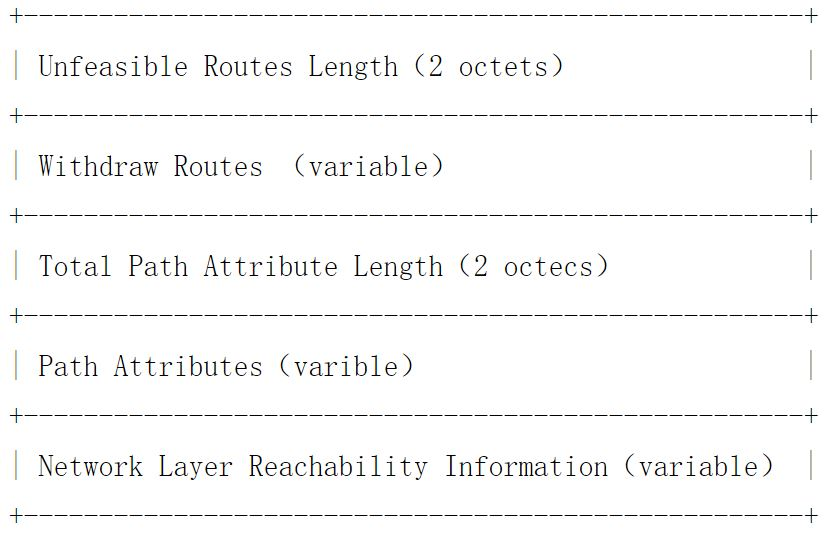
\includegraphics[width=0.6\textwidth]{updatemsg}
  \caption{UPDATE消息数据格式}
  \label{fig:updatemsg}
\end{figure}



\subsection{通信协议}
路由信息通过UPDATE消息在路由器之间进行传输。在本文提出的基于集中平台的iBGP新架构RSCP-iBGP中,需要将经过边界路由器Route-Client上的入站策略的路由信息传输到集中平台的Route-Server,包括路由信息中原本不在自治系统间传输的路由属性Weight,所以需要对自治系统内边界路由器上运行的BGP协议进行扩展:增加Path Attributes,从而能在自治系统内部通过扩展的iBGP协议传输附带Weight属性值的UPDATE路由信息。

BGP报文消息\cite{rfc4271}基于TCP协议进行传输,BGP消息主要由BGP头和数据部分组成。BGP消息报文的最大长度是4096字节,最小的BGP消息报文只包含BGP头没有数据仅19字节。BGP头部的长度为19字节,主要包含Marker、Length、Type三种类型的数据。BGP头部的Type字段主要标记BGP消息的类型:Type值为1表示OPEN消息,Type值为2表示UPDATE消息,Type值为3表示NOTIFICATION消息,Type值为4表示KEEPALIVE消息。

UPDATE消息主要用于BGP对等体之间宣告可达路由或者撤销不可达路由。BGP协议的UPDATE消息主要包含19字节的BGP头以及变长的UPDATE消息数据, 如图\ref{fig:updatemsg}。Path Attributes字段中记录了路由信息的属性,该字段由一个三元组组成<Attribute Type, Attribute Length, Attribute Value>。Attribute Type字段包含两部分Flag和Type Code。 Flag的长度为1个字节,前4位比特位取0或1,分别代表公认属性或可选属性、非传递属性或可传递属性、信息完整或信息不完整、属性长度为1字节或属性长度为2字节。已有的路径属性中的典型Type Code取值从1-7,分别对应路由信息的起源Origin、自治系统路径编号、Next\_hop值、MED属性值、Local Preference值、Atomic\_aggregate、Aggregate。

为了在自治系统间的iBGP连接中传输Weight属性,本文对Path Attributes的Attribute Type进行扩展,对传输Weight属性的Path Attribute三元组中涉及的元素进行设计:
\begin{itemize}
  \item Flag为01000000,表示Weight属性为公认属性则所有路由器均可识别,Weight属性为可传递属性,在RSCP-iBGP系统中需要从边界路由器传输到集中平台,信息是完整的,且属性长度是1字节;
  \item 设置传输Weight属性的Attribute Type Code为31(本文提出的RSCP-iBGP系统基于Quagga\cite{quagga}实现,目前Quagga中BGP协议实现的Attribute Type Code没有值为31的Path Attribute,增设路径属性Type Code值);
  \item Weight属性值的范围为 0-$(2^{16}-1)$,则传输Weight的Attribute Length值为2,转为16进制为0x02。
\end{itemize}

\section{对比分析}

为了解决iBGP可扩展问题,学术界提出了分布式路由体系结构下的路由反射和AS联邦,以及集中式路由体系结构下的SoftRouter、RCP、RFCP等5种解决方案。其5种方案虽然很好地解决了iBGP存在的可扩展问题,但存在新的隐患,比如分布式路由体系结构下的路由反射、AS联邦带来的非最优路由、路由震荡等问题;集中式路由体系结构下的SoftRouter、RCP以及RFCP并没有充分利用集中平台的结构优势,对路由存储和路由计算进行优化等。本文提出的RSCP-iBGP系统不仅解决了iBGP可扩展问题,且解决了现有的分布式路由体系结构方案存在的非最优路由、路由震荡等问题,优化了现有集中式路由体系结构方案没有优化的路由存储和路由计算,具体的对比分析如下:

\begin{figure}
  \centering
  % Requires \usepackage{graphicx}
  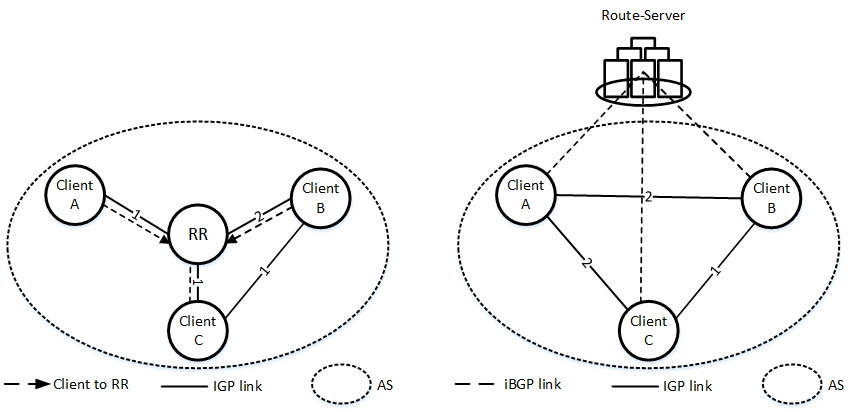
\includegraphics[width=0.75\textwidth]{rscp-best}
  \caption{解决路由反射引起的非最优出口举例}
  \label{fig:rscp-best}
\end{figure}


\subsection{解决iBGP可扩展问题}

假设某自治系统有N台边界路由器,在传统Full-Mesh的iBGP结构中,域内自治系统需要建立N\verb+*+(N-1)/2数量的BGP连接。该自治系统的拓扑结构对应到本文的RSCP-iBGP系统结构,自治系统内的有N台Route-Client边界路由器用于接受转发其他自治系统传输过来的路由、1台运行在集中平台的Route-Server用于路由存储和路由计算等操作,N台Route-Client与1台Route-Server建立N个扩展的iBGP连接来传输iBGP路由信息。iBGP连接数量下降了一个数量级,则该基于集中平台的RSCP-iBGP新架构解决了iBGP协议可扩展性差的问题。

\subsection{与分布式路由体系结构方案的对比}

学术界提出的2种比较典型的分布式路由体系结构方案分别是路由反射和AS联邦,具体的概念和存在的问题在第二章进行了详细的综述。本文提出的RSCP-iBGP系统没有路由反射中非最优出口、转发环路、路由震荡等问题,也没有AS联邦中非最优出口和路由震荡等问题。

\subsubsection{解决路由反射存在问题}



路由反射在特定情况下,因为最优路由计算缺少全部路由、结构设计不合理、MED值不可比等多方面原因,可能产生非最优路由、转发环路、路由震荡等问题。但在本文的RSCP-iBGP新系统中,路由计算基于全部的路由信息,不存在路由反射器仅将最优路由发送给客户机的情况。RSCP-iBGP系统中的复式路由计算采用集合缩小法而不是两两比较的路由算法,解决了MED值不可比的问题。RSCP-iBGP新系统有效地解决了路由反射中非最优路由、转发环路和路由震荡的问题,对比章节\ref{subsubsec:rr}的例子具体说明。\\

\begin{figure}
  \centering
  % Requires \usepackage{graphicx}
  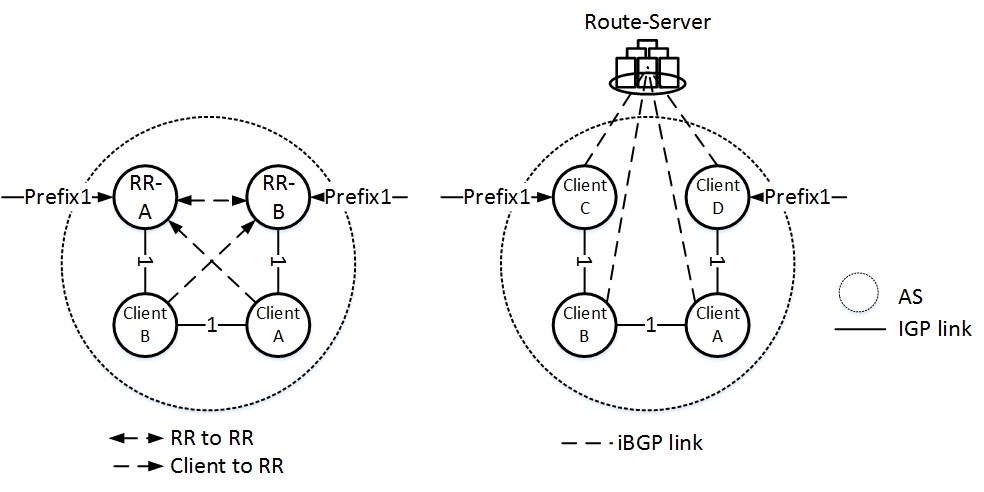
\includegraphics[width=0.9\textwidth]{rscp-noloop}
  \caption{解决路由反射引起的转发环路举例}
  \label{fig:rscp-noloop}
\end{figure}


\paragraph{路由反射引起的非最优路由}
在图\ref{fig:rscp-best}中,左侧为路由反射自治系统内的网络结构,右侧为RSCP-iBGP新系统下自治系统内的网络结构。Client-A和Client-B分别接收到一条eBGP路由,其来自同一AS,且前缀、Weight、Local Preference、As-path、MED值均相同。在RSCP-iBGP新系统中,Client-A和Client-B会将这两条路由传输到集中平台的Route-Server;Route-Server通过复式路由计算为自治系统内的3个边界路由器计算最优路由,因为这两条路由来自同一AS,且前缀、Weight、Local Preference、As-path、MED值均相同,则根据IGPcost进行路由选择,Client-A选择其自身接收到的eBGP路由作为该前缀的最优路由,Client-B选择其自身接收到的eBGP路由作为该前缀的最优路由,Client-C选择Client-B作为自己的最优出口,即Client-C选择Client-B从eBGP邻居收到的路由作为自己的最优路由。

RSCP-iBGP新系统解决了路由反射中的非最优路由问题,因为RSCP-iBGP新系统上所有边界路由器的最优路由计算都是基于全部的路由信息,所以计算结果均是理论上的最优路由。\\


\paragraph{路由反射引起的转发环路}

路由反射转发环路发生的原因是路由反射结构设置不合理,数据包在转发的过程中多次被重新路由。在RSCP-iBGP新系统中,如图\ref{fig:rscp-noloop},Client-C(对应路由反射器RR-A)和Client-D(对应路由反射器RR-B)会将其收到的路由信息传输给集中平台上的Route-Server,Client-C收到的路由记为Prefix1-route1, Client-D收到的路由标记为Prefix1-route2,Route-Server会经过复式路由计算模块计算出自治系统内的四台边界路由器的最优路由,Client-B的最优出口是Client-C,Client-A的最优出口是Client-D。当Client-B要发送目的地址为Prefix1的数据包时,直接通过Client-C转发出去,不会发生转发环路。\\

\begin{figure}
  \centering
  % Requires \usepackage{graphicx}
  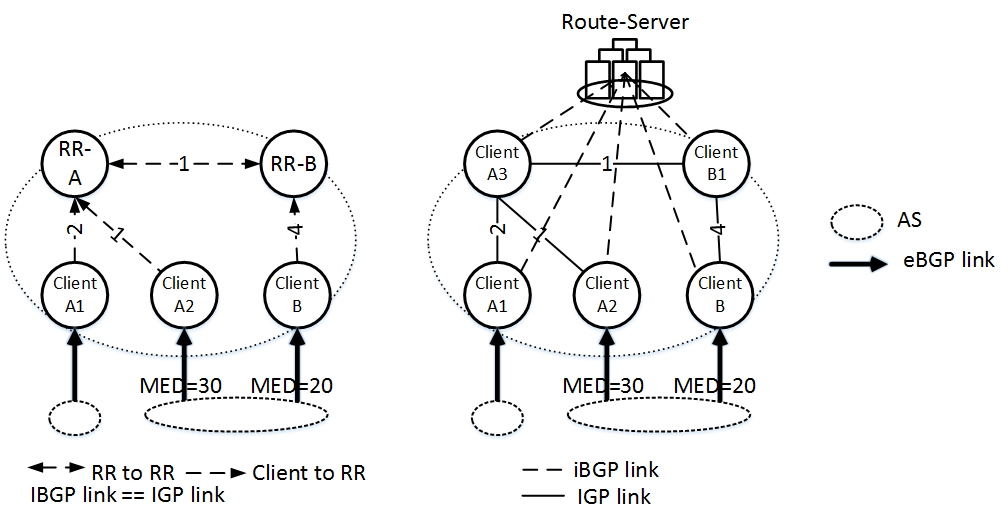
\includegraphics[width=0.9\textwidth]{rscp-nomed}
  \caption{解决路由反射引起的MED路由震荡举例}
  \label{fig:rscp-nomed}
\end{figure}


\paragraph{路由反射引起的MED震荡}

路由反射引起的MED震荡主要是因为某些时刻MED值不可比较,导致最优路由的结果发生变化,从而发生路由震荡。在图\ref{fig:rscp-nomed}中,左侧为路由反射结构中因为MED值发生路由震荡的网络拓扑,右侧为左侧对应的RSCP-iBGP新系统下自治系统内的网络拓扑。在RSCP-iBGP的新系统中,Client-A1、Client-A2、Client-B收到的3条路由均会传输到集中平台的Route-Server。因为传输到自治系统内的3条路由,前缀、Weight、Local Preference、As-path长度均相同。在Route-Server的复式路由计算模块中,对于域内的所有边界路由器,Client-B收到的eBGP路由优于Client-A2收到的eBGP路由,所以自治系统内的其他路由器的最优路由,根据IGPcost,在Client-A1收到的eBGP路由和Client-B收到的eBGP路由,这两条路由之间选择。在RSCP-iBGP新系统中,路由计算采用集合缩小法,基于全部的路由进行路由计算,并不会因为MED值产生路由震荡。\\


\begin{figure}
  \centering
  % Requires \usepackage{graphicx}
  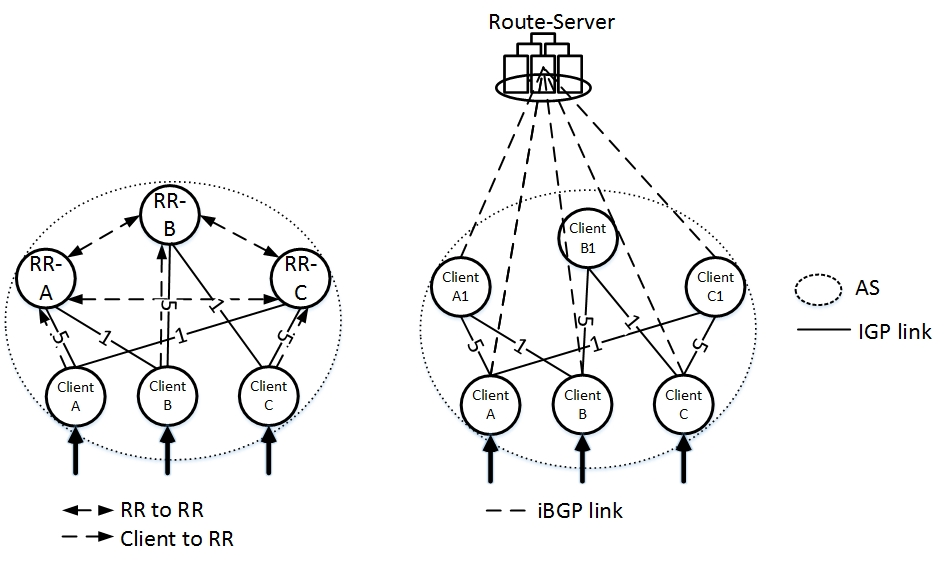
\includegraphics[width=0.9\textwidth]{rscp-notopo}
  \caption{解决路由反射引起的拓扑路由震荡举例}
  \label{fig:rscp-notopo}
\end{figure}

\paragraph{路由反射引起的拓扑震荡}

路由反射引起的拓扑震荡主要是因为路由反射结构设计不合理,路由决策主要依赖IGPcost值,一旦接收到其他路由反射器的最优路由,本身的最优路由会发生改变,将本身的最优路由宣告出去之后,会引起其他路由反射器最优路由的变化,最终导致路由震荡产生。在图\ref{fig:rscp-notopo}中,左侧路由反射结构中因为路由反射结构设计不合理发生路由震荡的网络拓扑,右侧为左侧对应的RSCP-iBGP新系统下自治系统内的网络拓扑。在RSCP-iBGP的新系统中,Client-A、Client-B、Client-C收到的3条路由均会传输到集中平台的Route-Server。因为传输到自治系统内的3条路由,前缀、Weight、Local Preference、As-path长度、MED均相同,则在Route-Server的复式路由计算模块中,主要依据IGPcost计算自治系统内的所有边界路由器的最优路由,Client-A1的最优出口是Client-B,Client-B1的最优出口是Client-C,Client-C1的最优出口是Client-A。在RSCP-iBGP新系统中,基于全部路由进行路由计算,解决了路由反射中路由反射器仅反射最优路由的特性以及路由反射拓扑设计等因素导致的路由震荡。

\subsubsection{解决AS联邦存在问题}


\begin{figure}
  \centering
  % Requires \usepackage{graphicx}
  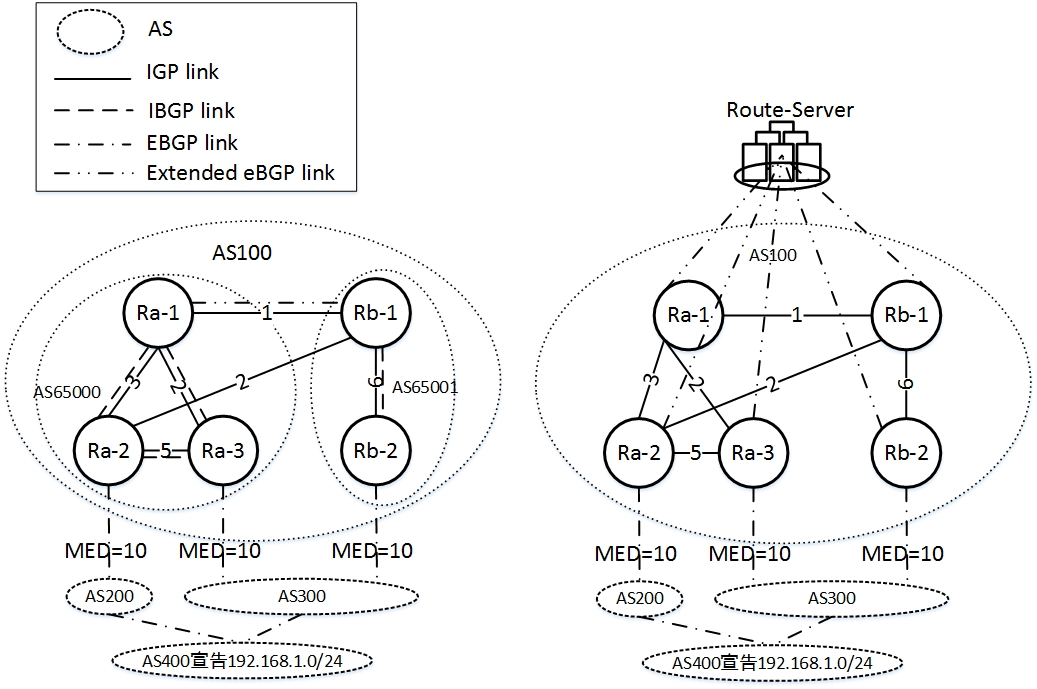
\includegraphics[width=0.9\textwidth]{rscp-asbest}
  \caption{解决AS联邦引起的非最优路由举例}
  \label{fig:rscp-asbest}
\end{figure}

AS联邦解决了iBGP可扩展问题,但在特定情况下也会产生路由计算非最优路由、路由震荡等问题。本文提出的RSCP-iBGP新系统,路由计算基于全部的路由信息,同时为自治系统内的所有边界路由器计算最优路由,没有路由收敛的过程,也不会出现AS联邦存在的隐患。\\

\paragraph{AS联邦引起的非最优路由}
AS联邦导致非最优路由的主要原因在于,自治系统内部的子自治系统之间仅传输最优路由,这直接导致某些子自治系统并没有全部的路由信息。在图\ref{fig:rscp-asbest}中,左侧为AS联邦结构中产生非最优路由情况的网络拓扑,右侧为左侧对应的RSCP-iBGP新系统下自治系统内的网络拓扑。在RSCP-iBGP的新系统中,Ra-2、Ra-3、Rb-2收到的3条由自治系统400向外宣告的192.168.1.0/24的路由信息,这3条路由信息均会传输到集中平台的Route-Server。因为传输到自治系统内的3条路由,前缀、Weight、Local Preference、As-path长度、MED均相同,则在Route-Server的复式路由计算模块中,主要依据IGPcost计算自治系统内的所有边界路由器的最优路由,Ra-1的最优出口是Ra-3,Rb-1的最优出口是Ra-2。在RSCP-iBGP新系统中,基于全部路由进行路由计算,解决了AS联邦的非最优路由问题。\\




\begin{figure}
  \centering
  % Requires \usepackage{graphicx}
  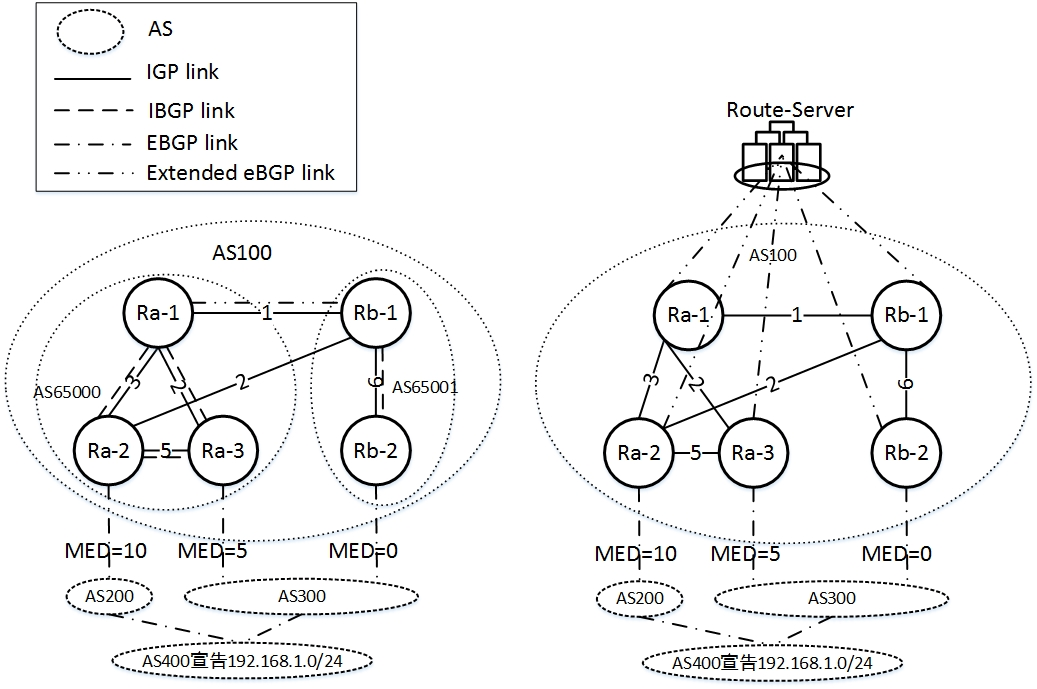
\includegraphics[width=0.9\textwidth]{rscp-asnomed}
  \caption{解决AS联邦引起的路由震荡举例}
  \label{fig:rscp-asnomed}
\end{figure}

\paragraph{AS联邦引起的路由震荡}

AS联邦导致的路由震荡主要原因在于,自治系统内部的子自治系统之间仅传输最优路由,且最优路由两两比较中MED不可比,这直接导致某些子自治系统向外宣告的最优路由会随着接收到的新路由信息产生变化,最后在路由收敛的过程中产生路由震荡。在图\ref{fig:rscp-asnomed}中,左侧为AS联邦结构中产生路由震荡的网络拓扑,右侧为左侧对应的RSCP-iBGP新系统下自治系统内的网络拓扑。在RSCP-iBGP的新系统中,Ra-2、Ra-3、Rb-2收到的3条由自治系统400向外宣告的192.168.1.0/24的路由信息,这3条路由信息均会传输到集中平台的Route-Server。因为传输到自治系统内的3条路由,前缀、Weight、Local Preference、As-path长度均相同,则在Route-Server的复式路由计算模块中,主要依据MED、IGPcost等计算自治系统内的所有边界路由器的最优路由。Route-Server的复式路由计算模块,采用集合缩小法,对于域内的所有边界路由器,Rb-2收到的eBGP路由优于Ra-3收到的eBGP路由,所以自治系统内的其他路由器的最优路由,主要根据IGPcost,在Ra-2收到的eBGP路由和Rb-2收到的eBGP路由,这两条路由之间选择。Ra-1的最优出口是Ra-2,Rb-1的最优出口是Ra-2,Ra-3的最优出口是Ra-3。在RSCP-iBGP新系统中,基于全部路由进行路由计算,且没有路由收敛的过程,解决了AS联邦的路由震荡问题。

\subsection{与集中式路由体系结构方案的对比}


学术界提出的3种比较典型的集中式路由体系结构方案分别是SoftRouter、RCP、RFCP,具体的概念和存在的问题在第二章进行了详细的综述。本文提出的RSCP-iBGP系统借鉴了集中式路由体系结构的概念,充分利用集中平台的资源和优势,对路由存储和路由计算进行了优化。

\subsubsection{SoftRouter}

本文提出的RSCP-iBGP新系统的结构,相对于SoftRouter中CE和FE多对多的结构要简单很多,其平台本身的可扩展性要比SoftRouter要好;SoftRouter中对路由存储和路由计算并没有进行优化,主要思想是将其控制平面与数据平面分离,而RSCP-iBGP新系统中对路由存储、路由计算都进行了优化,均优化了一个数量级单位的指标;SoftRouter容易开发部署新的功能,而本文提出的RSCP-iBGP拥有集中平台这一显著优势,也能充分利用集中平台的资源,在集中平台上部署更多的网络功能,加强路由协议的安全性以及配置路由策略的灵活性等。

\subsubsection{RCP}
RCP路由控制平台提出了集中式路由存储、策略配置、路由计算的思想,不仅在自治系统内部有集中控制平台,同时部署RCP的自治系统之间也能通过RCP的平台进行域间的信息传输。本文提出的RSCP-iBGP新系统,和RCP的基本思想相同,但具体实现有所差异。本文提出的RSCP-iBGP系统平台的可扩展性更强,注重解决iBGP的问题,且在集中平台上实现了路由计算、路由存储的优化。未来RSCP-iBGP也能充分利用集中平台的优势,实现路由策略的配置集中管理和优化、路由配置正确性检测等方案。


\subsubsection{RFCP}

RFCP是集中式收集路由信息,通过构建虚拟的拓扑环境模拟真实自治系统内的网络环境,将虚拟拓扑环境中Full-Mesh的分布式计算结果传输给真实的网络结构。RFCP的实现需要部署SDN的可编程式交换机,在自治系统内的运行SDN控制器上运行应用程序来进行路由计算,集中式的对路由信息进行管理。但其路由表在虚拟的拓扑环境中仍冗余存储,路由计算属于传统的分布式计算方法,策略配置仍需要在每台边界路由器上进行配置。RSCP-iBGP新系统与RFCP相比,存在很多优势,RSCP-iBGP系统不仅将路由存储空间和路由计算次数优化了一个数量级的标准。RSCP-iBGP系统中集中平台的优势和资源,也能帮助网络管理员更好地进行路由存储和路由计算。


\begin{table}[h]
	\centering
	\caption{RSCP-iBGP新系统与现有解决iBGP可扩展问题的相关研究的对比}
    \label{tab:compare}

    \begin{tabular}{@{}ccccccc@{}}
\toprule
关注点              & RR & AS联邦 & SoftRouter & RCP & RFCP & RSCP-iBGP \\ \midrule
路由可扩展性:不需要全连接    &  $\surd$ &  $\surd$  & $\surd$  &$\surd$ & $\surd$  &$\surd$       \\
路由计算:基于全部路由      &   $\times$ &  $\times$  & $\surd$  &$\surd$ & $\surd$  &$\surd$  \\
路由计算:no MED引起的震荡 & $\times$ &  $\times$  & $\surd$  &$\surd$ & $\surd$  &$\surd$  \\
路由计算次数优化         &   $\times$ &  $\times$  & $\times$  &$\times$ & $\times$  &$\surd$ \\
路由表集中存储          &  $\times$ &  $\times$  & $\surd$  &$\surd$ & $\times$  &$\surd$      \\
路由表村抽优化          & $\times$ &  $\times$  & $\times$  &$\times$ & $\times$  &$\surd$    \\ \bottomrule
\end{tabular}
\end{table}

\subsection{总结}

本章节主要论证本文提出的RSCP-iBGP新系统,相比于现有的学术界提出的2种分布式路由体系结构下的方案、3种集中式路由体系结构下的方案具有的优势,验证该方案的设计目标和价值意义。基于上述RSCP-iBGP系统与分布式路由体系结构和集中式路由体系结构的对比分析,可得到RSCP-iBGP系统与5种已有研究的概括性比较,如表\ref{tab:compare}所示。



\section{本章小结}

本文提出的RSCP-iBGP新系统不仅能解决iBGP存在的可扩展问题,而且能够基于全部的路由进行路由计算。在此基础上,RSCP-iBGP新系统利用集中平台的优势和资源,对传统的分布式的路由存储和路由计算进行了优化,将存储空间以及当存在路由更新时自治系统内的路由计算次数均优化了一个数量级的标准。本章节详细介绍了RSCP-iBGP的系统架构,边界路由器、集中平台、通信协议等RSCP-iBGP系统的三大部分、以及RSCP-iBGP系统与现有解决iBGP可扩展问题的相关研究进行了对比分析,论证了该RSCP-iBGP新系统的设计合理性、显著优势等理论。

